% PREAMBLE ====================================================================
% This borrows heavily from Christoph's template, but includes a few more helpful packages

\documentclass[11pt, letterpaper]{article}

% --- load packages ---
\usepackage{amsmath}       				% for equations
\usepackage{graphicx}      				% for figures
\usepackage[inner=2.5cm, 
			outer=2.5cm, 
			top=3cm, 
			bottom=3cm
			]{geometry} 				% adjust margins
\usepackage{subcaption} 				% allow subfigures
\usepackage{xcolor} 					% more colour choices
\usepackage{enumerate}					% for lists
\usepackage{float}						% specify locations of things
\usepackage[labelfont=bf]{caption}		% make all figure labels bold
\usepackage{parskip} 					% disable indenting of new paragraphs
\usepackage[section]{placeins} 			% place a figure in a section
\usepackage{enumitem} 					% resume numbering in lists with enumerate
\usepackage{dirtree} 					% create directory tree structures
\usepackage{hyperref} 					% create internal links in document

% change font
%\usepackage[T1]{fontenc}
%\usepackage{txfonts}

%\usepackage[T1]{fontenc}
%\usepackage{fourier}

% BODY ========================================================================
\begin{document}

% --- top matter ---

 % Use custom title	
\begin{center}
	\Large \textbf{WhaleMap}: A tool for collating and disseminating whale survey data in near real-time \\
	\bigskip
	\normalsize 18 December 2017 \\
	\normalsize Hansen Johnson and Pam Emery\\
	\bigskip
\end{center}

% abstract  
\begin{abstract}
	The survival of North Atlantic right whales (NARWs) relies on management decisions informed by visual and acoustic surveys. Effective communication of survey data within and between research, government, industry and the public is critical and lacking. Here we propose an automated system for collating and displaying survey data from all platforms and groups in near real-time. We cover some of the details of the system, provide some examples of its use and advantages, and outline steps required to make it operational for the 2018 field season in Atlantic Canada.
\end{abstract} 

% --- main matter ---

% Section 1 ------------------------------------------------------------------
\section{The problem: communication}

The unusual mortality event in the Gulf of St Lawrence (GoSL) in 2017 prompted unprecedented survey effort in the region and brought global attention to the urgency of NARW conservation. The events of last year also place extraordinary importance on the 2018 field season in Atlantic Canada, which we anticipate will be the most comprehensive to date. The resources and attention devoted to this cause are phenomenal and warranted, but bring with them a unique set of challenges. 

One such challenge is clear: we need a system to rapidly and efficiently disseminate survey information within and between research, government, industry, and public sectors. This is crucial for three key reasons. First, communication among survey teams allows dynamic response to the latest information, which maximizes survey efficiency. Second, communication between survey teams, government regulators, and industry stakeholders expedites informed, transparent management decisions. Third, making this information available to the media and broader public raises awareness and reduces the spread of misinformation. 

In the past, when the community was relatively small and/or localized, a daily or weekly email list (i.e., the `MarWhales' list administered by DFO Maritimes) was sufficient to share information. As the user community grew to include more researchers, DFO regions, industries, and more, `MarWhales' became too unwieldy and inefficient to keep everyone informed in a timely manner.  The email list became problematic for two reasons. The first problem was that all the incoming survey data, information requests, quality control, outgoing emails, and other associated work all fell to a single DFO employee with other responsibilities. The timeliness of the updates fell entirely on them and their ability to juggle their other responsibilities. The second set of issues arose from sending data (either as maps or tables of lat/lon positions) out to the listserv. Relinquishing direct control over the data in this way made it difficult to correct errors and maintain consistency in the dataset. These formats were also difficult to extract meaningful information from. The urgency of NARW conservation, importance of effective communication, and inefficiency of previous communication mechanisms propel us towards alternative tools for the 2018 season.

% Section 2 ------------------------------------------------------------------
\newpage
\section{A solution: WhaleMap}

\subsection{Overview}

We have developed a tool to address the problem of timely data dissemination. It was designed to 1) operate with minimal supervision or impact on survey teams, 2) allow data originators to retain complete control over their data, and 3) provide the latest data in a user-friendly, accessible format. 

The system, which we're calling \textbf{WhaleMap}, is essentially a computer program that pulls in data from each survey team, combines these data into a single, cohesive format, constructs interactive maps of all available information, and hosts the maps online. Figure 1 provides a conceptual overview of the \textbf{WhaleMap} workflow, which can be broken down into two steps. First, survey teams upload raw data to a designated shared folder in a remote repository of their choice (e.g., Google Drive, Dropbox, etc). Second, the host server (currently at Dalhousie University) automatically ingests the new data, adds it to the existing database, and rebuilds the interactive online maps. The server frequently checks remote repositories for updates and repeats step two anytime a change is made in any of the watched folders.

\begin{figure}[h]
	\centering
	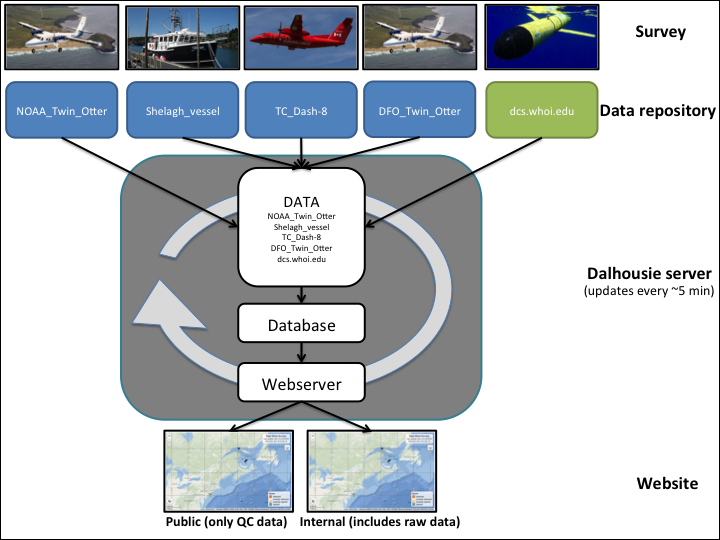
\includegraphics[width=0.7\linewidth]{diagram}
	\caption{Overview of the \textbf{WhaleMap} workflow}
	\label{fig:outline}
\end{figure}

\subsection{Advantages}

\subsubsection{Efficiency}

The \textbf{WhaleMap} system eliminates the requirement for a person to mediate the dissemination of the latest information. It also has several features designed to minimize impacts on the survey teams. First, it to synchronize with remote repositories because virtually every survey team already uses a system like Google Drive or Dropbox to organize and share their data. Second, it does not require survey teams to change the format in which they collect their data. Instead, it is capable of ingesting and collating data in a variety of forms, which avoids imposing a standardized system on each survey team. The results of these features mean that survey teams need to merely upload their data onto their Google Drive or Dropbox folder, as they normally do, and the results becomes nearly instantly viewable online.

\subsubsection{Data control}

Critically, \textbf{WhaleMap} reacts to changes made to the raw data in each survey team's remote repository. For example, if a member of a given team catches an error, removes a file, or performs some level of quality control, the online map will update to reflect the change. This is very important because it allows each survey team to retain direct control over their data. It is also important to note that raw data will never be made openly available online. All the produced maps are `view-only', meaning that it will not be possible for anyone to download the data directly from \textbf{WhaleMap}. All data requests will need to be made via the data originators.

\subsubsection{Accessibility}

Perhaps the greatest benefit of \textbf{WhaleMap} is its ability to consolidate all data streams and make them available in a user-friendly format in a single location. Instead of requesting the latest data from DFO or relying on a potentially outdated static map, an interested stakeholder can simply refer to a single source for the latest information. Furthermore, interactive online maps are an incredibly powerful way to view and gain intuition from data. The maps produced by \textbf{WhaleMap} are designed to be user-friendly and intuitive, with controls to zoom in and out, measure distances, draw, view metadata, turn data layers off/on, and more. All of these features attempt to maximize the usability of the data. 

Some concerns have arisen regarding the widespread sharing of data that has not been quality controlled. This is particularly critical with aerial surveys that often generate a large number of duplicate sightings. \textbf{WhaleMap} can overcome this issue by producing two separate online maps, one that is publically available containing only quality controlled data, and a second for internal use (e.g., password protected or secret link) that includes all raw data. A great benefit of \textbf{WhaleMap} is that virtually every aspect of the system can be tailored to meet our specific needs. It is, first and foremost, a tool built by scientists for scientists. 

\subsection{Requirements}

We have relied entirely on established, open source tools that are well-established in the scientific community (e.g. the R programming language) so that the system can be implemented at virtually no cost by researchers without extensive programming experience.

Aside from the software development, the success of this tool depends entirely upon each survey platform using a \textbf{consistent}, \textbf{documented}, format for their data. We're not suggesting that everyone adopt a single system. Each group is free to use whatever format works best for them, but must consistent in their choice. Figures 2 and 3 in the Appendix show examples of formats previously used by survey teams on the NOAA Twin Otter and CWI Shelagh, respectively. Either of these systems, and many others, are perfectly amenable to our proposed system, provided they remain consistent throughout the field season.

\subsection{Current status and next steps}

\subsubsection{Online demonstration}

The framework for \textbf{WhaleMap} has already been tested and developed. A demonstration of the trial version is currently live at \url{https://leviathan.ocean.dal.ca}. The main page of this site would be analogous to the `public' map described previously, while the link to the \textbf{WhaleMap} (on the task bar at the upper right, or via \url{https://leviathan.ocean.dal.ca/WhaleMap}), is a more comprehensive map system that could be available (via password or secret link) for internal use only. Example screenshots from each map are available in the Appendix. 

\subsubsection{Next steps}

First, we need to get input from each potential survey team to determine: 1) the data format they intend to use during the 2018 field season (with examples and documentation), 2) how we should deal with the issue of quality control for their dataset, and 3) how we could improve or adjust the system to meet their needs. We then need to implement the suggestions made by the survey groups, and write source code required to process all anticipated data formats. The latter should be easily achievable if formats remain relatively consistent from 2017. If we start now, we will be able to complete and test the system before fieldwork begins in the spring of 2018.

\subsubsection{The future}

All of this work has been done with the hope that this system, or something like it, can be used in the long term. The immediate need for such a system prompted us to build and house it at Dalhousie, but we are aware that it cannot reside there indefinitely. With this in mind, we have made all source code and documentation openly available at \url{https://github.com/hansenjohnson/WhaleMap}. This GitHub repository could be used to easily migrate the entire system to a new host location, or be a resource for future developers to use when building a more permanent or sustainable system.

% Section ------------------------------------------------------------------
\newpage
\section{Appendix}

\subsection{Data examples}

\begin{figure}[H]	
	\dirtree{%
		.1 Google Drive.
		.2 /NOAA\_Twin\_Otter\DTcomment{Shared Google Drive folder}.
		.3 /170622\DTcomment{All data for June 22, 2017}.
		.3 /170627\DTcomment{All data for June 27, 2017}.
		.3 /170710\DTcomment{All data for July 10, 2017}.
		.4 170710.sig\DTcomment{Sightings data}.
		.4 170710.gps\DTcomment{Track data}.
		.4 170710.eff\DTcomment{Effort data}.
	}
	\caption{Example directory structure of NOAA survey data.}
\end{figure}

\begin{figure}[H]	
	\dirtree{%
		.1 Google Drive.
		.2 /Shelagh\_Data\DTcomment{Shared Google Drive folder}.
		.3 2017-07-10-CWI-V-FINAL.csv\DTcomment{Sightings and effort thru Jul 10, 2017 [leg 1]}.
		.3 2017-08-12-CWI-V-FINAL.csv\DTcomment{Sightings and effort thru Aug 12, 2017 [leg 2]}.
	}
	\caption{Example directory structure of Shelagh survey data.}
\end{figure}

\subsection{Screenshots}

\begin{figure}[H]
	\centering
	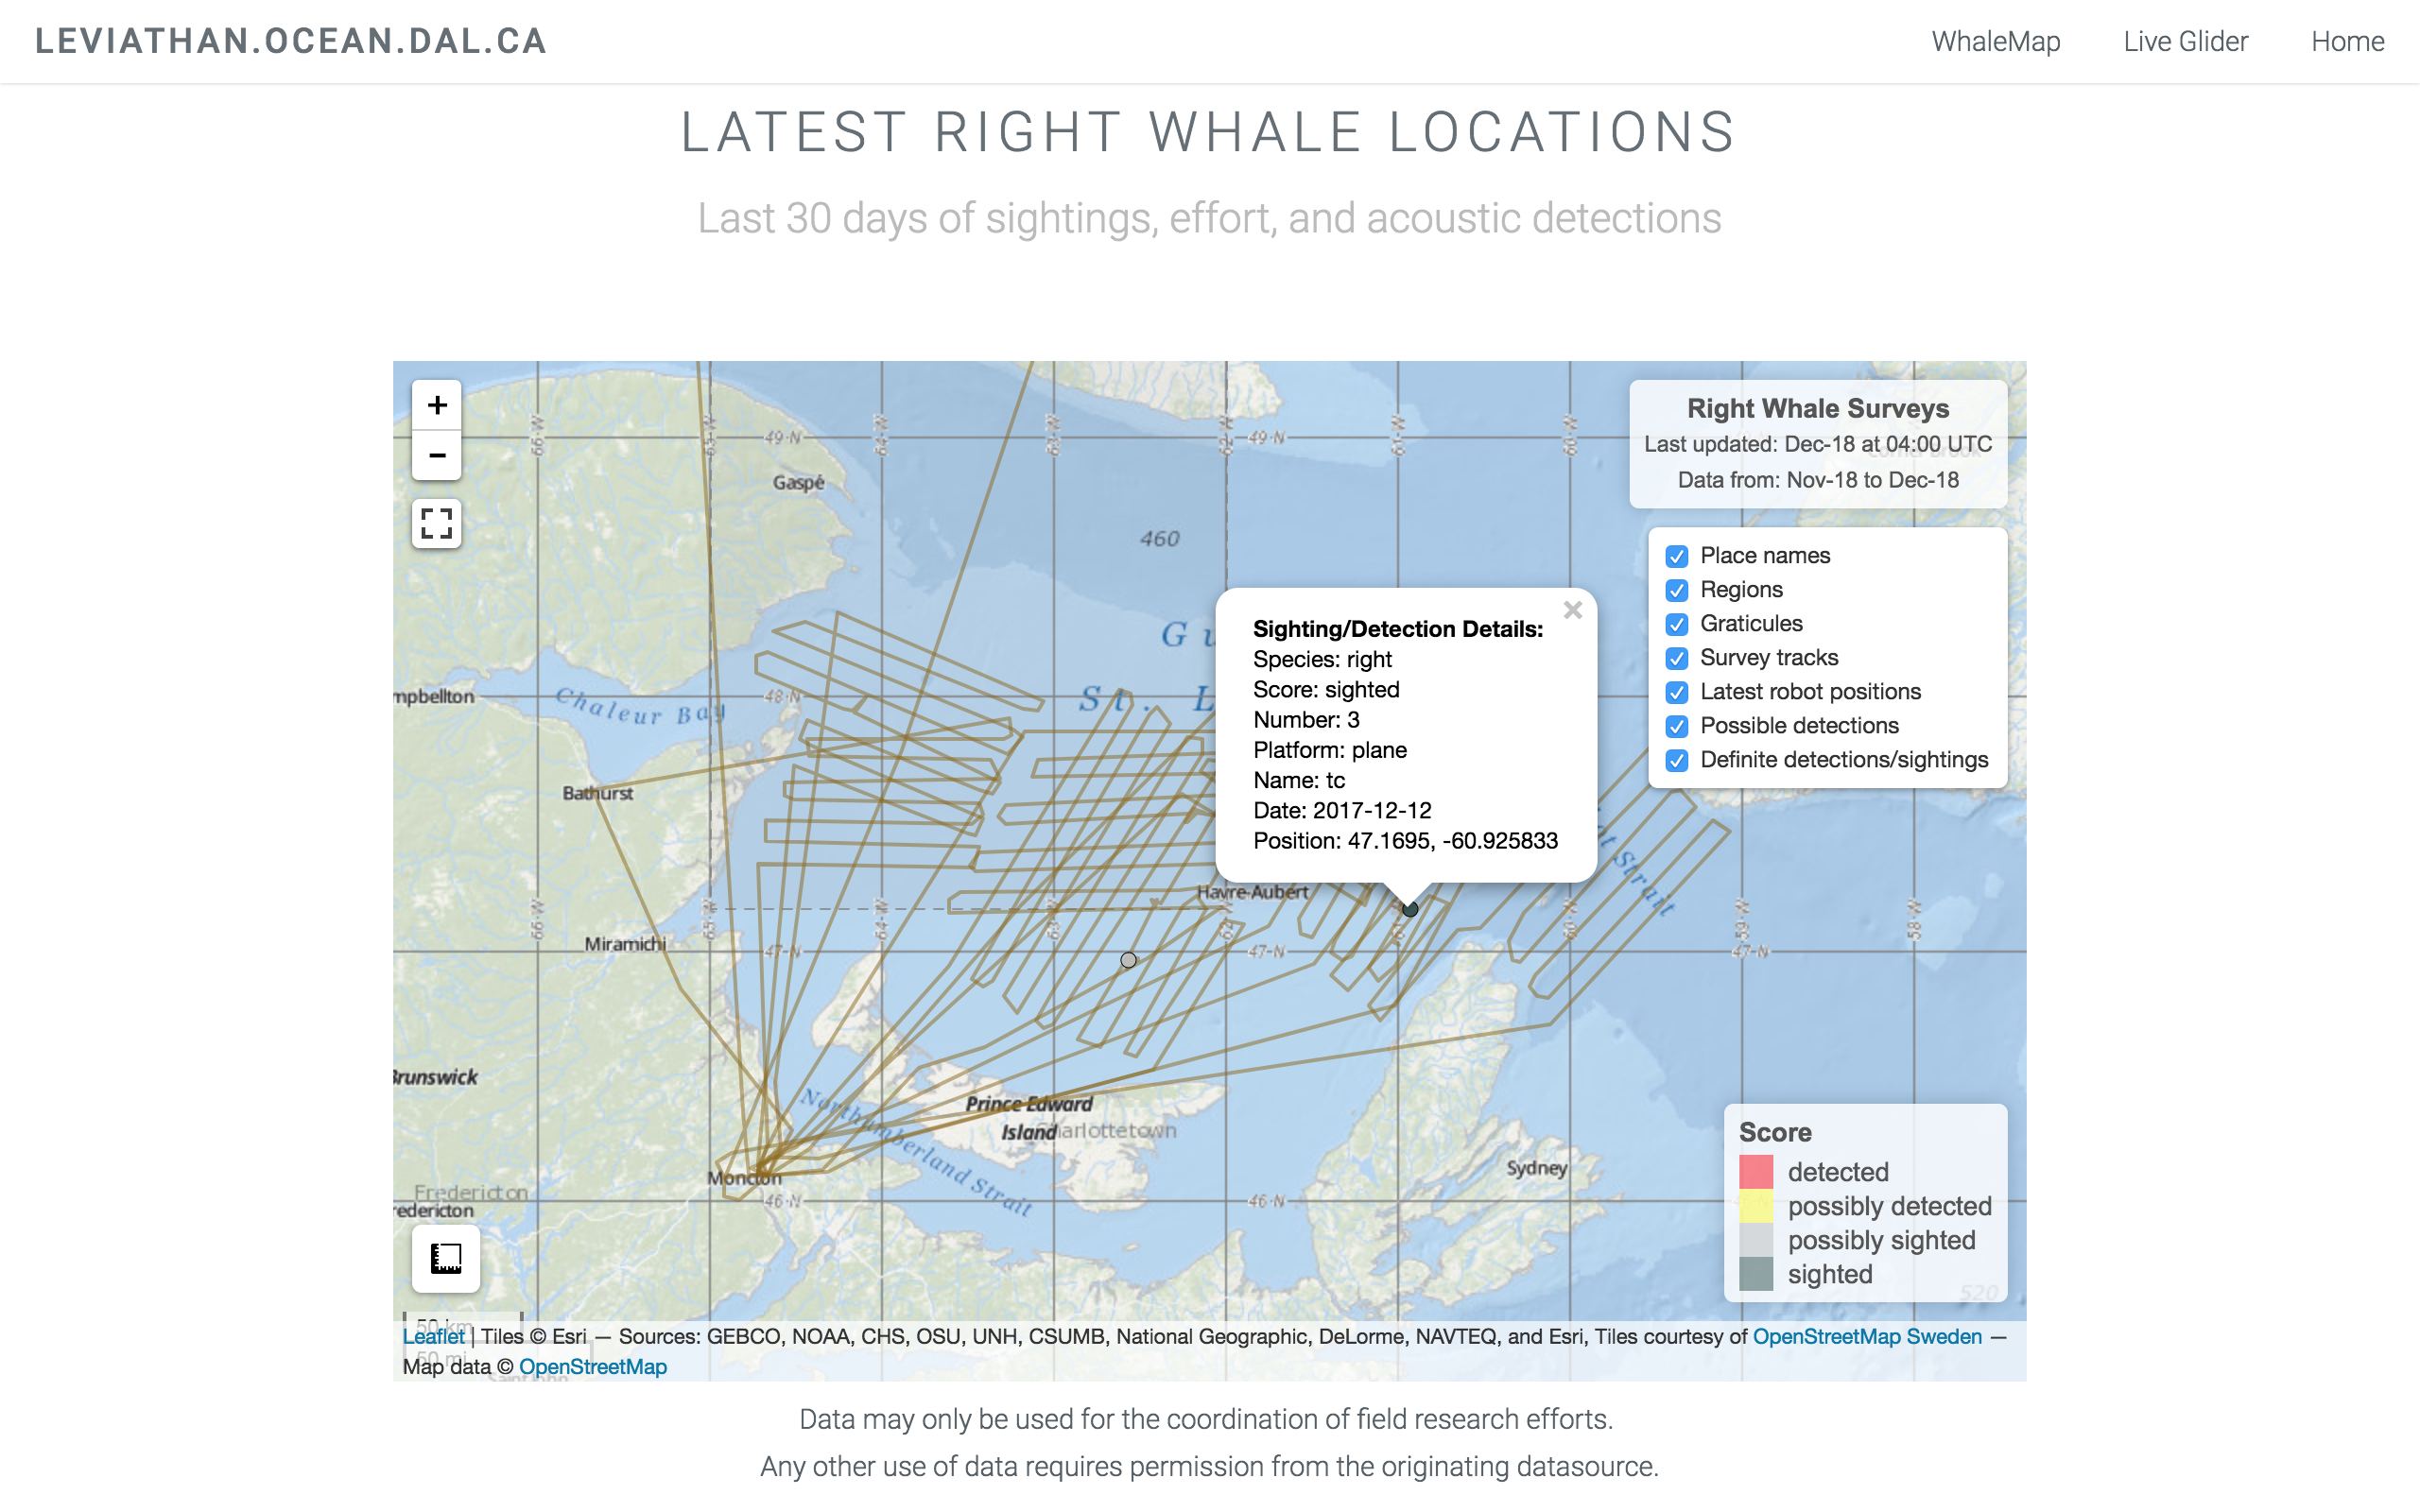
\includegraphics[width=0.7\linewidth]{public_zoom}
	\caption{Screenshot of the `public facing' interactive survey map showing the effort in the GoSL over the last month, with a sighting selected to illustrate information conveyed ( taken from \url{https://leviathan.ocean.dal.ca/} on Dec 18, 2017)}
	\label{fig:publiczoom}
\end{figure}

\begin{figure}[H]
	\centering
	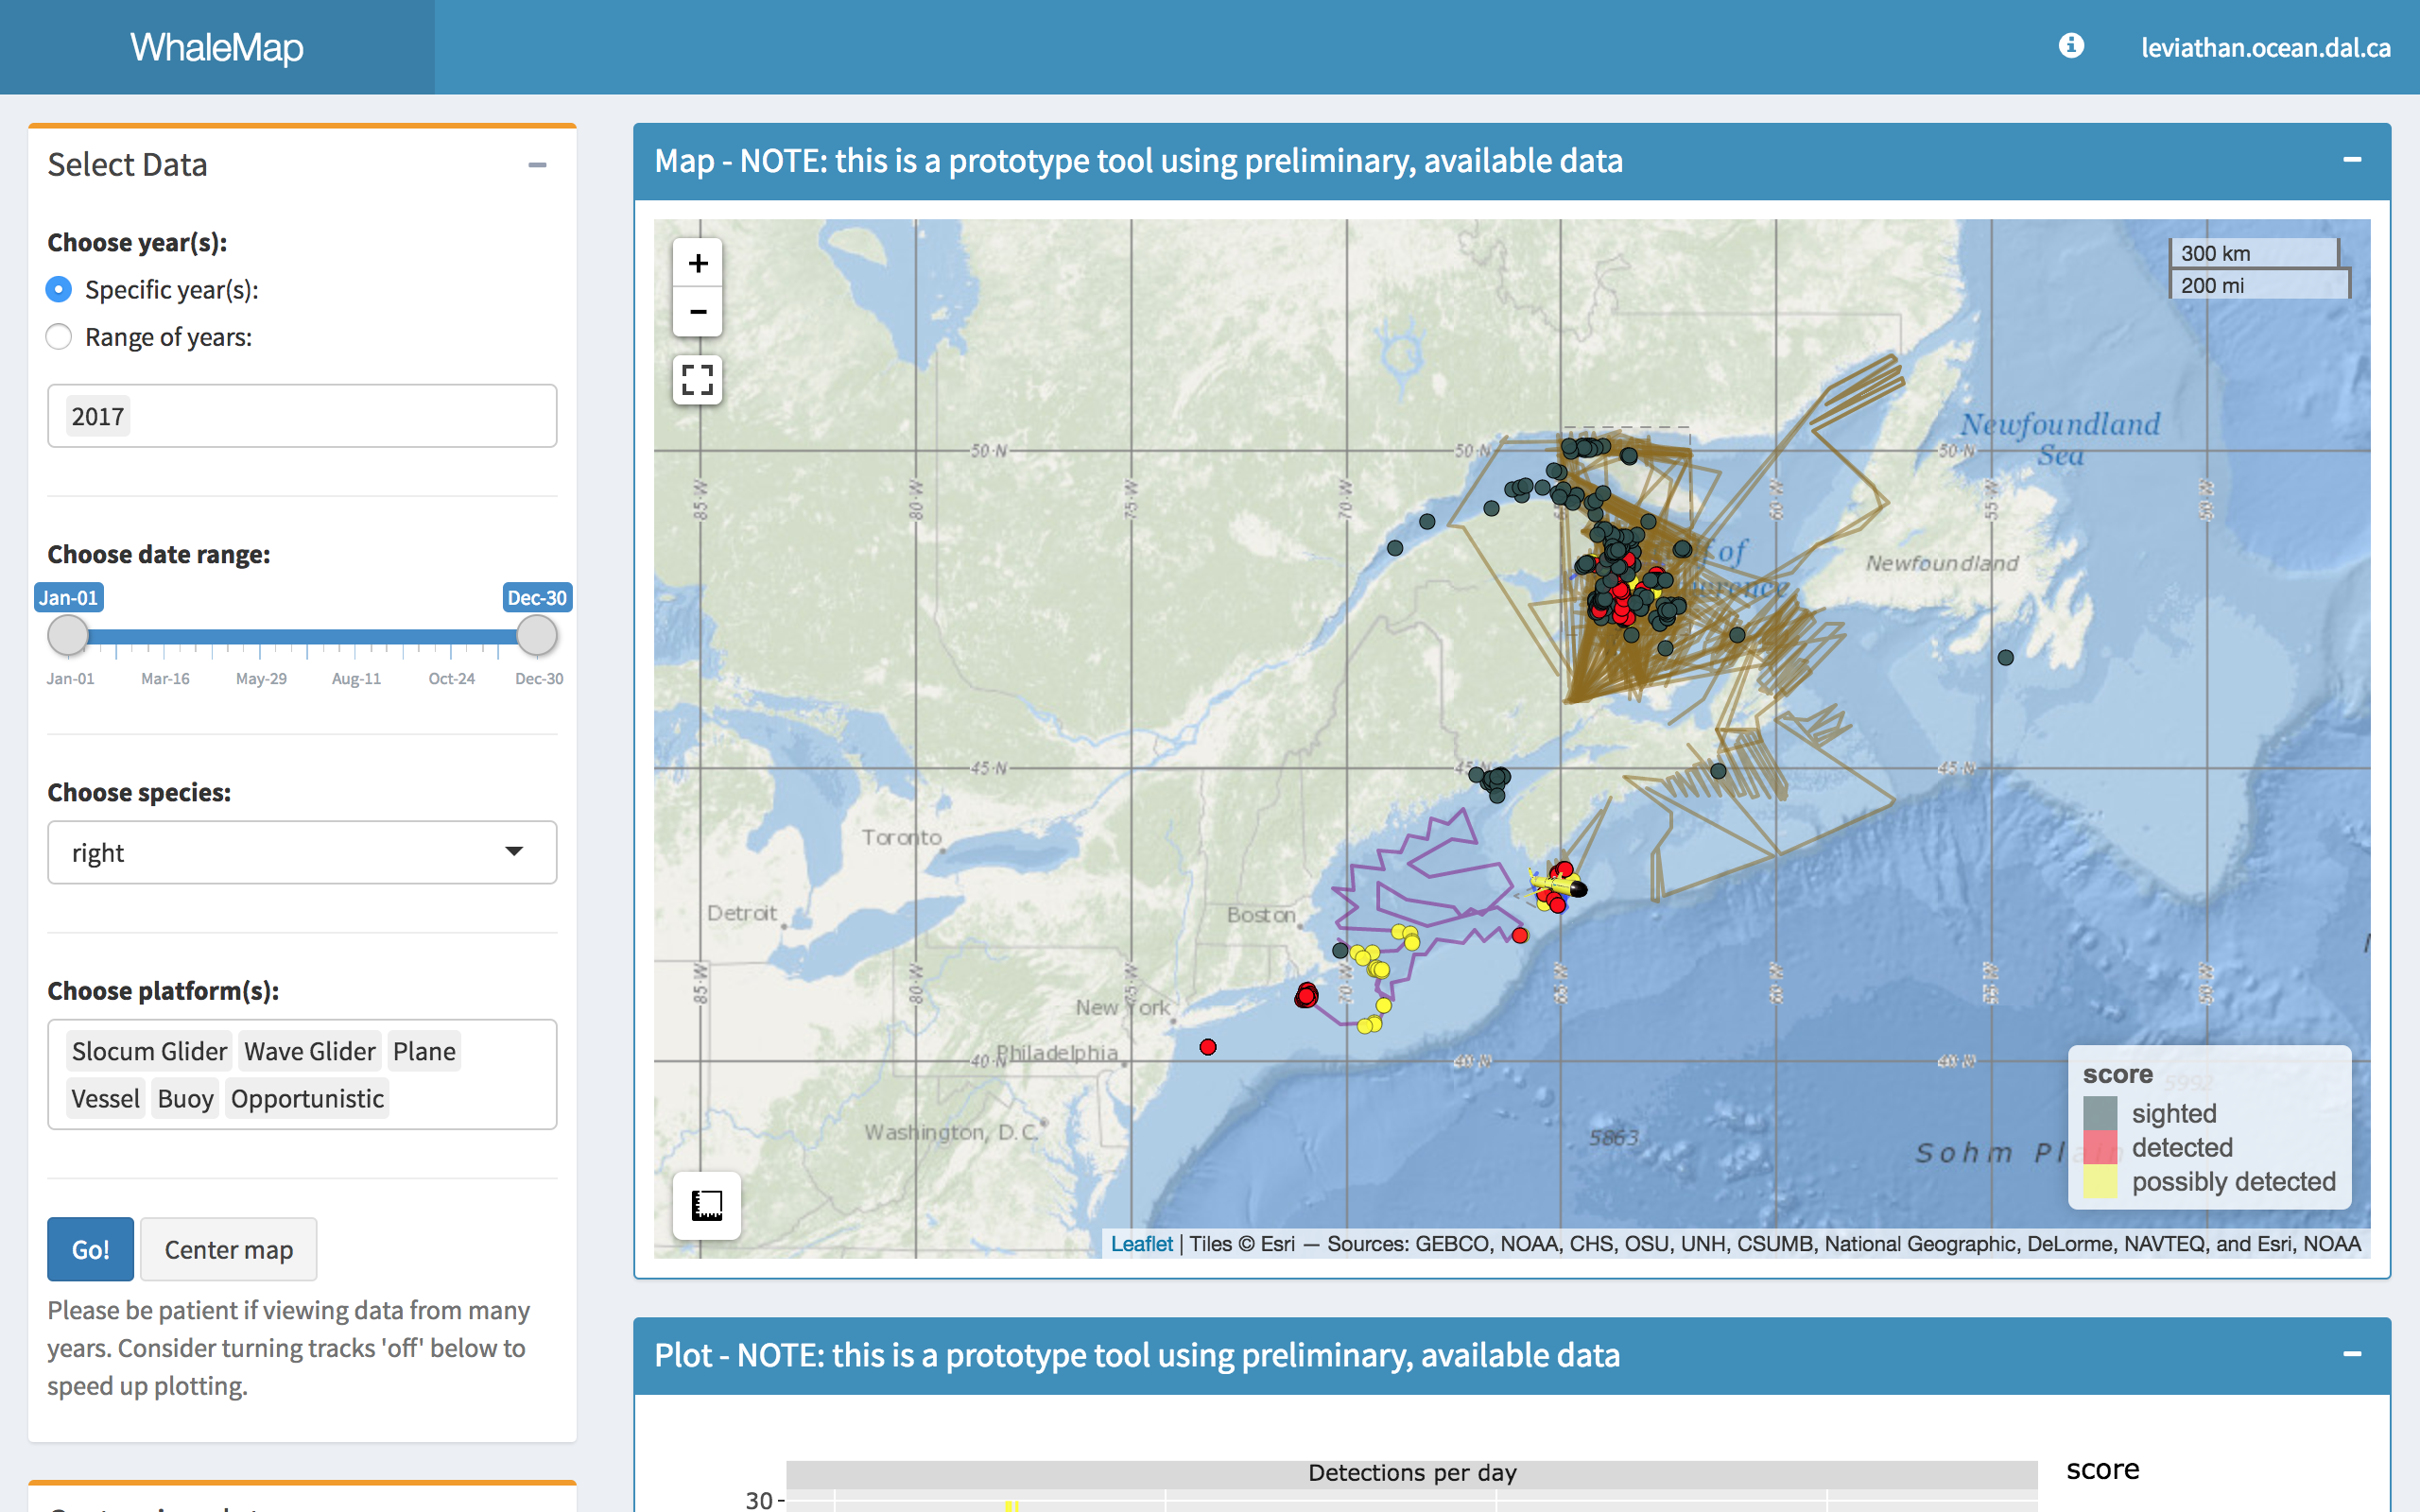
\includegraphics[width=0.7\linewidth]{WhaleMap_all}
	\caption{Screenshot of the `internal use' interactive survey map application showing all survey effort in 2017 (taken from \url{https://leviathan.ocean.dal.ca/WhaleMap} on Dec 18, 2017)}
	\label{fig:whalemapall}
\end{figure}

\subsection{Links}

\begin{description}
	\item[Public map:] \url{https://leviathan.ocean.dal.ca	}
	\item[Internal map:] \url{https://leviathan.ocean.dal.ca/WhaleMap}
	\item[Help for internal map:] \url{http://leviathan.ocean.dal.ca/leviathan_docs/WhaleMap-help.html}
	\item[Source code:] \url{https://github.com/hansenjohnson/WhaleMap}
	\item[Issue tracking:] \url{https://github.com/hansenjohnson/WhaleMap/issues}
\end{description}

% --- back matter ---
% e.g. bibliography (not covered here)

\end{document}